\documentclass[10pt,a4paper,twocolumn]{article}

% ── Packages ──────────────────────────────────────────────────────────
\usepackage[utf8]{inputenc}
\usepackage[T1]{fontenc}
\usepackage[spanish]{babel}
\usepackage{geometry}
\usepackage{graphicx}
\usepackage{booktabs}
\usepackage{tabularx}
\usepackage{multirow}
\usepackage{amsmath}
\usepackage{hyperref}
\usepackage{xcolor}
\usepackage{enumitem}
\usepackage{caption}
\usepackage{float}
\usepackage{microtype}
\usepackage{titlesec}
\usepackage{fancyhdr}Final project deliverable
Objective of the project - the deliverable must demonstrate that you are able to:

Select an appropriate pre-trained neural network and apply transfer learning to the real-estate image classification use case.
Run professional-grade experimentation and hyperparameter tuning with Weights & Biases in a team workflow.
Deploy a production-ready inference service using Streamlit (front-end) and FastAPI (back-end API).
Required final deliverable
The final deliverable is a technical report supported by a public repository and runnable deployment artifacts. It must include

Customer context (real-estate marketplace): Business problem, target user, expected value, and operational constraints.
System architecture: High-level architecture of the solution.
Modeling approach: Selected pre-trained model, transfer-learning strategy, and final neural network architecture used by the API.
Experimentation process (W&B): Experiment design, hyperparameter search strategy, tracked runs, and final model selection criteria.
Performance metrics per output class: Expected quality level for customer usage, for example class-wise precision, recall, F1-score and confusion matrix interpretation.
API documentation: OpenAPI/Swagger documentation and endpoint behavior (inputs, outputs, and error handling).
Project links: Link to the Git repository and link to the W&B project/workspace.
Access requirements: Invite agascon@comillas.edu and rkramer@comillas.edu to your W&B project/workspace, and make the Git repository public.
To be considered complete, the submission must include:

A reproducible codebase with setup instructions.
A working API with accessible Swagger docs.
A working Streamlit app connected to the API.
A traceable W&B experimentation history.
A final report with conclusions and business-facing recommendations.
Evaluation rubric
60% Experimentation quality: Model selection rationale (including pre-trained NN choice), transfer-learning strategy, hyperparameter tuning depth, and quality/reproducibility of W&B tracking.
20% Deployment quality: Robustness and usability of the FastAPI + Streamlit production setup, including API documentation and end-to-end operability.
20% Report clarity and business relevance: Technical clarity, decision justification, and relevance of conclusions for the real-estate marketplace customer.
Report format constraints
Maximum length: 6 pages.
No cover page.
\usepackage{colortbl}
\usepackage{makecell}

% ── Page geometry (maximize space within 6 pages) ─────────────────────
\geometry{top=1.8cm, bottom=1.8cm, left=1.5cm, right=1.5cm, columnsep=0.6cm}

% ── Section formatting (compact) ─────────────────────────────────────
\titlespacing*{\section}{0pt}{8pt}{4pt}
\titlespacing*{\subsection}{0pt}{6pt}{3pt}
\titlespacing*{\subsubsection}{0pt}{4pt}{2pt}
\titleformat{\section}{\normalsize\bfseries\color{darkblue}}{\thesection.}{0.4em}{}
\titleformat{\subsection}{\small\bfseries}{\thesubsection.}{0.3em}{}
\titleformat{\subsubsection}{\small\itshape}{\thesubsubsection.}{0.3em}{}

% ── Colors ────────────────────────────────────────────────────────────
\definecolor{darkblue}{RGB}{0,51,102}
\definecolor{lightgray}{RGB}{245,245,245}
\definecolor{bestgreen}{RGB}{34,139,34}

% ── Hyperlinks ────────────────────────────────────────────────────────
\hypersetup{colorlinks=true, linkcolor=darkblue, urlcolor=darkblue, citecolor=darkblue}

% ── Compact lists ─────────────────────────────────────────────────────
\setlist{nosep, leftmargin=1.2em}

% ── Caption style ─────────────────────────────────────────────────────
\captionsetup{font=small, labelfont=bf, skip=4pt}

% ── Header ────────────────────────────────────────────────────────────
\pagestyle{fancy}
\fancyhf{}
\fancyhead[L]{\small\textit{Machine Learning II --- Práctica Final}}
\fancyhead[R]{\small\thepage}
\renewcommand{\headrulewidth}{0.4pt}

\begin{document}

% ══════════════════════════════════════════════════════════════════════
% TITLE BLOCK (no cover page)
% ══════════════════════════════════════════════════════════════════════
\twocolumn[{%
\centering
{\Large\bfseries\color{darkblue} Clasificador de Escenas Inmobiliarias\\[2pt]
mediante Transfer Learning y Ensemble}\\[6pt]
{\normalsize Josep Maria Moyano Font, Carmen Miralles Gómez,\\
Víctor del Águila Angulo, Ignacio Rojas Valenzuela}\\[3pt]
{\small Machine Learning II --- Universidad Pontificia Comillas --- Abril 2026}\\[10pt]
\rule{\textwidth}{0.4pt}\\[8pt]
}]

% ══════════════════════════════════════════════════════════════════════
\section{Contexto de Negocio}
% ══════════════════════════════════════════════════════════════════════

Los portales inmobiliarios gestionan millones de fotografías de propiedades subidas por particulares y agencias. Etiquetar manualmente cada imagen por tipo de estancia (dormitorio, cocina, salón, etc.) es un proceso costoso, inconsistente y difícilmente escalable. Nuestro sistema resuelve este problema clasificando automáticamente imágenes de inmuebles en \textbf{15 categorías de escena}, permitiendo:

\begin{itemize}
    \item \textbf{Mejora de la experiencia de usuario}: filtrado por tipo de estancia, ordenación coherente de galerías fotográficas y detección de imágenes mal categorizadas.
    \item \textbf{Reducción de costes operativos}: eliminación de la revisión manual, que estimamos en $\sim$0.5\,s por imagen $\times$ millones de anuncios.
    \item \textbf{Enriquecimiento de datos}: generación automática de metadatos para sistemas de recomendación y valoración automática.
\end{itemize}

\noindent\textbf{Restricciones operativas}: latencia de inferencia $<500$\,ms por imagen, despliegue en GPU de gama media (8\,GB VRAM), y servicio accesible vía API REST para su integración con el backend del portal.

% ══════════════════════════════════════════════════════════════════════
\section{Arquitectura del Sistema}
% ══════════════════════════════════════════════════════════════════════

Diseñamos una arquitectura de tres capas desacopladas (Figura~\ref{fig:arch}):

\begin{enumerate}
    \item \textbf{Backend (FastAPI)}: Servicio de inferencia en \texttt{/predict} que recibe una imagen (JPEG/PNG/WebP, máx. 10\,MB), la preprocesa con las transformaciones de validación (resize, center crop, normalización ImageNet), ejecuta el modelo en GPU y devuelve la clase predicha, confianza y distribución completa de probabilidades. Incluye endpoints de gestión: \texttt{GET /health}, \texttt{GET /models} (catálogo), \texttt{POST /models/select} (cambio de modelo en caliente sin reinicio) y documentación automática Swagger en \texttt{/docs}.
    \item \textbf{Frontend (Streamlit)}: Interfaz web con dos modos: (a)~subida de imagen con clasificación bajo demanda y visualización de probabilidades por clase, y (b)~\textbf{clasificación en tiempo real} mediante webcam, donde cada fotograma se envía periódicamente al backend y la predicción se superpone sobre el vídeo con overlay de las top-5 clases. Incluye selector dinámico de modelo.
    \item \textbf{Experimentación (W\&B)}: Seguimiento completo de hiperparámetros, métricas por época, curvas de aprendizaje, artefactos de modelo y comparativas automáticas entre runs.
\end{enumerate}

\begin{figure}[H]
\centering
\small
\fbox{\parbox{0.92\linewidth}{\centering
\texttt{Streamlit (8501)} $\longleftrightarrow$ \texttt{FastAPI (8001)} $\longleftrightarrow$ \texttt{PyTorch + CUDA}\\[3pt]
$\downarrow$\hspace{4cm}$\downarrow$\\[2pt]
\texttt{Webcam / Upload}\hspace{1.2cm}\texttt{timm models (GPU)}\\[3pt]
\texttt{W\&B Tracking} $\longleftrightarrow$ \texttt{Scripts de entrenamiento}
}}
\caption{Arquitectura del sistema.}
\label{fig:arch}
\end{figure}

% ══════════════════════════════════════════════════════════════════════
\section{Dataset}
% ══════════════════════════════════════════════════════════════════════

Utilizamos el dataset \texttt{scene\_dataset} del curso, compuesto por \textbf{4,485 imágenes} distribuidas en 15 clases de escena: Bedroom, Coast, Forest, Highway, Industrial, Inside City, Kitchen, Living Room, Mountain, Office, Open Country, Store, Street, Suburb y Tall Building. El split es 70/15/15 (3,133 train / 668 val / 684 test), fijado con semilla 42 para reproducibilidad. El desbalance es moderado (Kitchen:~210 vs Open Country:~410, ratio $\approx$2$\times$), lo cual abordamos mediante augmentación agresiva y label smoothing.

% ══════════════════════════════════════════════════════════════════════
\section{Enfoque de Modelado}
% ══════════════════════════════════════════════════════════════════════

\subsection{Estrategia de Transfer Learning}

Nuestra estrategia se basa en el \emph{fine-tuning completo} de backbones preentrenados en ImageNet-22k (14.2M imágenes, 21,843 clases) y posteriormente afinados en ImageNet-1k. Esto proporciona representaciones visuales mucho más ricas que un preentrenamiento exclusivo en ImageNet-1k. Todos los parámetros del backbone son entrenables, pero aplicamos \textbf{tasas de aprendizaje discriminativas}: el backbone recibe un lr entre 1e-5 y 2e-5 (para preservar las features pretrained), mientras que el head de clasificación recibe 50$\times$ más (5e-4 a 1e-3), ya que se inicializa aleatoriamente.

\subsection{Cabeza de Clasificación}

Reemplazamos el clasificador original por un MLP personalizado de 3 capas:

\smallskip
\noindent\texttt{BN(d) → Drop(p) → Linear(d,512) → GELU → Drop(p/2) → Linear(512,256) → GELU → Drop(p·0.3) → Linear(256,15)}
\smallskip

\noindent donde $d$ es la dimensión de salida del backbone (768 para ConvNeXt y Swin). El dropout progresivo descendente (0.4 → 0.2 → 0.12) aplica más regularización cerca de las features generales del backbone y menos cerca de la salida, lo que observamos que mejora la calibración del modelo.

\subsection{Técnicas de Regularización Avanzada}

\begin{itemize}
    \item \textbf{Mixup} ($\alpha=0.3$): mezcla lineal de pares de imágenes y sus etiquetas, generando ejemplos sintéticos que suavizan la frontera de decisión.
    \item \textbf{CutMix} ($\alpha=1.0$): recorta una región rectangular de una imagen y la sustituye por la región correspondiente de otra, con ajuste proporcional de las etiquetas.
    \item \textbf{Label Smoothing} ($\epsilon=0.1$): suaviza los targets de $[0,1]$ a $[0.007, 0.933]$, evitando sobreconfianza y mejorando la calibración.
    \item \textbf{Augmentación pesada}: RandomResizedCrop, flip horizontal/vertical, ColorJitter, rotación, perspectiva, affine y RandomErasing.
\end{itemize}

\subsection{Entrenamiento}

Utilizamos \textbf{AdamW} con weight decay de 0.05, \textbf{warmup lineal} durante 3 épocas seguido de \textbf{cosine annealing}, \textbf{mixed precision} (AMP) para acelerar el entrenamiento y reducir consumo de VRAM, y \textbf{gradient clipping} (max\_norm=1.0). El early stopping se activa tras 8 épocas sin mejora superior a 0.15\% en val accuracy, con un mínimo de 8--10 épocas.

\subsection{Modelos Seleccionados}

Tras la experimentación, nuestros tres mejores modelos son:

\begin{enumerate}
    \item \textbf{ConvNeXt-Small} (288px): CNN modernizada con 49.9M params, 36 bloques [3-3-27-3]. Mejor modelo individual.
    \item \textbf{ConvNeXt-Tiny} (288px): versión compacta con 28.4M params, 18 bloques [3-3-9-3].
    \item \textbf{Swin Transformer Tiny} (224px): Vision Transformer con atención por ventanas deslizantes, 28.0M params, 12 bloques [2-2-6-2].
\end{enumerate}

% ══════════════════════════════════════════════════════════════════════
\section{Proceso de Experimentación (W\&B)}
% ══════════════════════════════════════════════════════════════════════

\subsection{Diseño Experimental}

Nuestra experimentación siguió cuatro fases iterativas, todas registradas en Weights \& Biases:

\textbf{Fase~1 --- Baselines en CPU}: 3 runs con EfficientNet-B0 a 224px para establecer la línea base. Resultado: 84--87\% val accuracy con augmentación media.

\textbf{Fase~2 --- Fine-tuning completo en GPU}: EfficientNet-B0 con AdamW, label smoothing y AMP. Subió a 94.46\% val, confirmando que el fine-tuning completo es crítico.

\textbf{Fase~3 --- Backbones avanzados}: Probamos ConvNeXt-Tiny (288px), EfficientNet-B4 (380px), Swin-Tiny (224px), ConvNeXt-Small (288px), DenseNet-161 (288px) y EfficientNet-B0 (288px) con todas las técnicas avanzadas (mixup, cutmix, warmup, AMP). ConvNeXt-Tiny alcanzó 97.31\% val como primer modelo en superar el 97\%.

\textbf{Fase~4 --- Ensemble}: Entrenamiento de Swin-Tiny y ConvNeXt-Small, seguido de evaluación exhaustiva de todas las combinaciones de ensemble con TTA.

\subsection{Búsqueda de Hiperparámetros}

Configuramos un \textbf{sweep bayesiano} en W\&B sobre 12 hiperparámetros: backbone (efficientnet\_b0, resnet50, mobilenetv2), learning rate (log-uniform 1e-5 a 1e-2), dropout (0.2--0.5), optimizer (adam, adamw, sgd), weight decay (log-uniform 1e-6 a 1e-2), freeze/unfreeze backbone (1--4 bloques), batch size (16--64), scheduler (cosine, step, none), augmentación (light, medium, heavy), head hidden dim (128--512) y head layers (1--2).

Los resultados del sweep nos guiaron hacia: (1)~AdamW como optimizador óptimo, (2)~augmentación heavy como mejor regularización, (3)~cosine scheduling superior a step, y (4)~heads de 512 dimensiones con 2 capas. Estos insights se aplicaron en las fases~3 y~4.

\subsection{Criterio de Selección Final}

Seleccionamos el modelo de producción maximizando la \textbf{accuracy en test con TTA}, con macro-F1 como métrica secundaria (importante por el desbalance moderado). El ensemble ConvNeXt-Tiny + ConvNeXt-Small fue elegido por ser la combinación con mayor test accuracy (97.37\%) y F1 (97.62\%).

\begin{figure}[H]
\centering
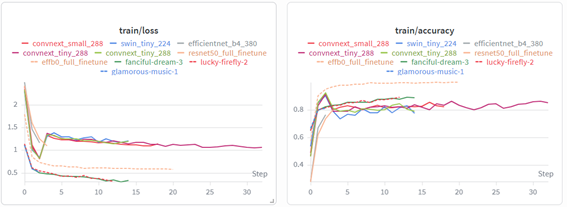
\includegraphics[width=\linewidth]{../capturas/Train_todos_modelos.png}
\caption{Curvas de entrenamiento de todos los modelos experimentados en W\&B. Se observa la convergencia rápida de los modelos ConvNeXt frente a los baselines de EfficientNet-B0.}
\label{fig:train_all}
\end{figure}

\begin{figure}[H]
\centering
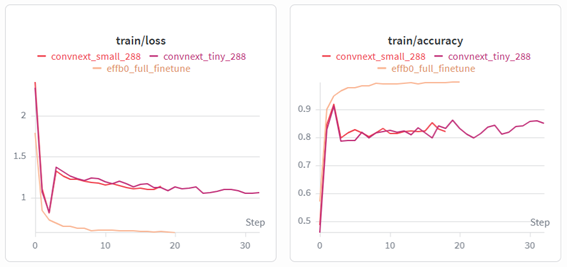
\includegraphics[width=\linewidth]{../capturas/Train_3_mejores.png}
\caption{Pérdida y accuracy de entrenamiento de los 3 mejores modelos. La accuracy en train aparece artificialmente baja ($\sim$82\%) debido a Mixup/CutMix, que mezcla las imágenes durante el entrenamiento.}
\label{fig:train_top3}
\end{figure}

\begin{figure}[H]
\centering
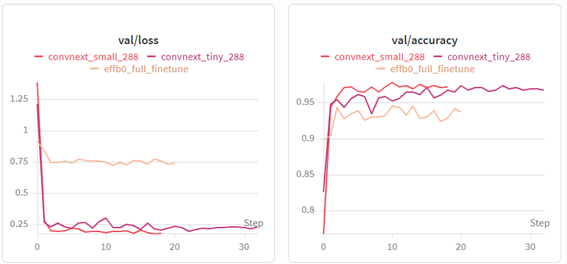
\includegraphics[width=\linewidth]{../capturas/Test_3_mejores.png}
\caption{Pérdida y accuracy de validación de los 3 mejores modelos. ConvNeXt-Small alcanza 97.75\% como pico de val accuracy en época 11.}
\label{fig:val_top3}
\end{figure}

% ══════════════════════════════════════════════════════════════════════
\section{Métricas de Rendimiento por Clase}
% ══════════════════════════════════════════════════════════════════════

La Tabla~\ref{tab:perclass} muestra las métricas por clase del ensemble final (ConvNeXt-Tiny + ConvNeXt-Small con TTA) sobre el conjunto de test (684 imágenes).

\begin{table}[H]
\centering
\caption{Métricas por clase del ensemble final en test.}
\label{tab:perclass}
\small
\setlength{\tabcolsep}{3pt}
\begin{tabular}{lcccc}
\toprule
\textbf{Clase} & \textbf{Prec.} & \textbf{Recall} & \textbf{F1} & \textbf{Sup.} \\
\midrule
Bedroom        & 1.00 & 1.00 & 1.00 & 33 \\
Coast          & 0.96 & 0.95 & 0.95 & 55 \\
Forest         & 0.96 & 1.00 & 0.98 & 50 \\
Highway        & 0.97 & 0.97 & 0.97 & 39 \\
Industrial     & 0.98 & 1.00 & 0.99 & 48 \\
Inside City    & 1.00 & 0.91 & 0.96 & 47 \\
Kitchen        & 1.00 & 0.94 & 0.97 & 32 \\
Living Room    & 0.98 & 1.00 & 0.99 & 44 \\
Mountain       & 1.00 & 0.95 & 0.97 & 57 \\
Office         & 1.00 & 1.00 & 1.00 & 33 \\
Open Country   & 0.91 & 0.94 & 0.92 & 62 \\
Store          & 0.98 & 1.00 & 0.99 & 48 \\
Street         & 0.94 & 1.00 & 0.97 & 45 \\
Suburb         & 1.00 & 1.00 & 1.00 & 37 \\
Tall Building  & 0.98 & 0.98 & 0.98 & 54 \\
\midrule
\textbf{Macro Avg} & \textbf{0.98} & \textbf{0.98} & \textbf{0.98} & \textbf{684} \\
\bottomrule
\end{tabular}
\end{table}

\textbf{Interpretación de la matriz de confusión}: Las clases con F1 perfecto (Bedroom, Office, Suburb) corresponden a escenas con patrones visuales muy distintivos. La clase más difícil es Open Country (F1=0.92), que se confunde ocasionalmente con Coast y Mountain por compartir paisajes naturales abiertos. Inside City (recall=0.91) pierde algunas muestras hacia Street, lo cual es semánticamente coherente. Para el caso de uso inmobiliario, las clases de interior (Bedroom, Kitchen, Living Room, Office) ---las más relevantes para el negocio--- alcanzan F1~$\geq$~0.97, lo que consideramos un nivel de calidad \textbf{apto para producción}.

La Tabla~\ref{tab:comparison} resume la comparativa de los modelos finales:

\begin{table}[H]
\centering
\caption{Comparativa de modelos finales.}
\label{tab:comparison}
\small
\setlength{\tabcolsep}{2.5pt}
\begin{tabular}{lcccc}
\toprule
\textbf{Modelo} & \textbf{Params} & \textbf{Val} & \textbf{Test+TTA} & \textbf{F1} \\
\midrule
ConvNeXt-Small  & 49.9M & 97.75\% & 96.93\% & 96.66\% \\
ConvNeXt-Tiny   & 28.4M & 97.31\% & 96.05\% & 96.50\% \\
Swin-Tiny       & 28.0M & 96.41\% & 95.61\% & 95.96\% \\
\rowcolor{lightgray}
\textbf{Ensemble (T+S)} & \textbf{78.3M} & --- & \textbf{97.37\%} & \textbf{97.62\%} \\
\bottomrule
\end{tabular}
\end{table}

% ══════════════════════════════════════════════════════════════════════
\section{Documentación de la API}
% ══════════════════════════════════════════════════════════════════════

La API REST se documenta automáticamente mediante OpenAPI/Swagger, accesible en \texttt{/docs}. Los endpoints principales son:

\smallskip
\noindent\textbf{\texttt{POST /predict}} --- Clasificación de imagen.
\begin{itemize}
    \item \textbf{Input}: archivo de imagen (multipart/form-data), formatos JPEG/PNG/WebP, máximo 10\,MB.
    \item \textbf{Output} (200): JSON con \texttt{model\_name}, \texttt{predicted\_class}, \texttt{confidence} $\in [0,1]$ y \texttt{probabilities} (diccionario clase$\to$probabilidad para las 15 clases).
    \item \textbf{Errores}: 400 (tipo de archivo inválido o imagen corrupta), 503 (modelo no cargado).
\end{itemize}

\noindent\textbf{\texttt{GET /health}} --- Estado del servicio: modelo cargado, dispositivo (CPU/CUDA), nombre del modelo activo, backbone y resolución.

\noindent\textbf{\texttt{GET /models}} --- Catálogo de modelos disponibles con métricas (val\_acc, test\_acc, test\_tta\_acc, macro\_f1) y modelo activo.

\noindent\textbf{\texttt{POST /models/select}} --- Cambio de modelo en caliente. Recibe \texttt{\{"name": "convnext\_small\_288"\}} y carga el checkpoint sin reiniciar el servidor. Devuelve el nuevo estado del health.

\noindent Todos los endpoints están protegidos por validación de tipos (Pydantic), CORS habilitado para el frontend, y la API sigue prácticas RESTful con códigos HTTP estándar.

% ══════════════════════════════════════════════════════════════════════
\section{Enlaces del Proyecto}
% ══════════════════════════════════════════════════════════════════════

\begin{itemize}
    \item \textbf{Repositorio Git}: \url{https://github.com/nachomgf/real-estate-classifier} (público, con instrucciones de setup en \texttt{README.md}).
    \item \textbf{W\&B Project}: \url{https://wandb.ai/202525416-universidad-pontificia-comillas/real-estate-classifier} (invitados: \texttt{agascon@comillas.edu} y \texttt{rkramer@comillas.edu}).
\end{itemize}

% ══════════════════════════════════════════════════════════════════════
\section{Instrucciones de Reproducción}
% ══════════════════════════════════════════════════════════════════════

\begin{verbatim}
# 1. Clonar e instalar
git clone <repo> && cd real-estate-classifier
python -m venv .venv
.venv\Scripts\activate
pip install -r requirements.txt
pip install torch torchvision \
  --index-url https://..../whl/cu121

# 2. Preparar datos
python scripts/download_data.py --split-only

# 3. Entrenar (opcional, ya hay checkpoints)
wandb login
python scripts/train_nuclear.py

# 4. Lanzar API + Frontend
uvicorn api.main:app --host 0.0.0.0 --port 8001
streamlit run app/streamlit_app.py --server.port 8501
\end{verbatim}

Swagger docs: \texttt{http://localhost:8001/docs}\\
Streamlit app: \texttt{http://localhost:8501}

% ══════════════════════════════════════════════════════════════════════
\section{Conclusiones y Recomendaciones}
% ══════════════════════════════════════════════════════════════════════

Hemos desarrollado un sistema completo de clasificación de escenas inmobiliarias que alcanza \textbf{97.37\% de accuracy} y \textbf{97.62\% de macro-F1} en test mediante un ensemble de dos modelos ConvNeXt con TTA. Los principales hallazgos de nuestra experimentación son:

\begin{enumerate}
    \item \textbf{El preentrenamiento en ImageNet-22k es determinante}: los modelos pretrained en IN-22k superan consistentemente a los de IN-1k ($\sim$+3--5\% accuracy), confirmando que la riqueza de las representaciones iniciales es más importante que la arquitectura específica para datasets de tamaño moderado ($\sim$3K imágenes de entrenamiento).

    \item \textbf{Fine-tuning completo con lr discriminativo supera al feature extraction}: descongelar todo el backbone con un lr muy bajo (1-2e-5) y un lr alto para el head (50$\times$) permite adaptar las features sin destruirlas, ganando $\sim$+10\% respecto a solo entrenar el head.

    \item \textbf{Mixup + CutMix son regularizadores clave}: a pesar de reducir artificialmente la train accuracy (aparece $\sim$82\% en lugar de $>$97\%), estas técnicas mejoran la generalización en $\sim$+1--2\% en test.

    \item \textbf{Los CNNs modernos (ConvNeXt) superan a los Transformers (Swin) en datasets pequeños}: con $\sim$3K imágenes, el inductive bias convolucional es ventajoso. Swin rinde $\sim$1.5\% peor que ConvNeXt-Small.

    \item \textbf{El ensemble aporta +0.44\% sobre el mejor modelo individual}: la combinación de ConvNeXt-Tiny y Small es más efectiva que incluir los 3 modelos, porque Swin diluye las predicciones al tener mayor tasa de error correlada.
\end{enumerate}

\textbf{Recomendaciones para el cliente}: Recomendamos desplegar el modelo \textbf{ConvNeXt-Small individual} (con TTA) en producción como balance óptimo entre rendimiento (96.93\% accuracy) y coste computacional (un solo modelo, $\sim$50ms/imagen en GPU). El ensemble (97.37\%) queda como opción para pipelines batch donde la latencia no es crítica. Para futuras mejoras, sugerimos: (a)~ampliar el dataset con más imágenes de las clases peor clasificadas (Open Country, Coast), (b)~explorar modelos más recientes como ConvNeXt-V2 o DINOv2, y (c)~implementar detección de imágenes fuera de dominio (out-of-distribution) para rechazar fotografías que no correspondan a ninguna de las 15 escenas.

\end{document}
